\documentclass[11pt,a4paper]{article}
\usepackage[T1]{fontenc}
\usepackage[utf8]{inputenc}
\usepackage{lmodern}
\usepackage{textcomp}
\usepackage[left=1.8cm,right=1.8cm,top=2.3cm,bottom=2.2cm,headheight=14pt,headsep=8pt]{geometry}
\usepackage{multicol}
\usepackage{xcolor}
\usepackage{fancyhdr}
\usepackage{graphicx}
\usepackage{array}
\usepackage{amsmath,amssymb}
\usepackage{setspace}
\usepackage{longtable}
\graphicspath{{../}}
\definecolor{ygreen}{RGB}{46,139,87}
\renewcommand{\normalsize}{\fontsize{10.9}{13.4}\selectfont}
\renewcommand{\familydefault}{\rmdefault}
\setlength{\parindent}{0pt}
\setlength{\columnsep}{0.8cm}
\setlength{\columnseprule}{0.4pt}
\setlength{\multicolsep}{3pt plus 1pt minus 1pt}
\renewcommand{\textsubscript}[1]{\ensuremath{_{\text{\fontsize{8}{8}\selectfont #1}}}}
\renewcommand{\textsuperscript}[1]{\ensuremath{^{\text{\fontsize{8}{8}\selectfont #1}}}}
\newcommand{\diqqat}[1]{\par\smallskip\noindent\textbf{Diqqat!} #1\par\medskip}
\newcommand{\javob}{\par\smallskip\noindent\textbf{Javob:} \rule[-2pt]{7.5cm}{0.4pt}\par\smallskip\noindent\textbf{Diqqat!} Javobingizni javoblar varaqasiga ko`chirib yozing.\par\medskip}
\pagestyle{fancy}
\fancyhf{}
\renewcommand{\headrulewidth}{0.4pt}
\fancyhead[L]{\textit{Milliy sertifikat 2026. Kimyo}}
\fancyhead[R]{14-variant}
\fancyfoot[L]{\fontsize{8}{9}\selectfont \textcopyright{} Colba maktabi, 2026}
\fancyfoot[C]{\thepage}
\fancypagestyle{first}{\fancyhf{}\renewcommand{\headrulewidth}{0pt}\fancyfoot[L]{\fontsize{8}{9}\selectfont \textcopyright{} Colba maktabi, 2026}\fancyfoot[C]{\thepage}}
\begin{document}
\normalsize
\thispagestyle{first}
\noindent\fcolorbox{ygreen}{white}{\parbox{\dimexpr\linewidth-2\fboxsep-2\fboxrule\relax}{%
\textbf{\fontsize{13}{15}\selectfont Nazorat testi}\ \textit{\fontsize{10}{12}\selectfont $\cdot$ Aralash test $\cdot$ 14-variant}\hfill
\begin{tabular}[t]{@{}r@{}}\textit{Milliy sertifikat 2026. Kimyo}\\ \textbf{\textit{\fontsize{8}{9}\selectfont Vaqt:}} \textit{\fontsize{10}{12}\selectfont 180 daqiqa}\end{tabular}}}
\par\medskip
\noindent\textit{Davriy jadvaldan foydalanish mumkin.}
\par\medskip
\begin{multicols}{2}
\noindent\textbf{1.} Rasmda molekulaning elektron (Lyuis) formulasi berilgan.
\begin{center}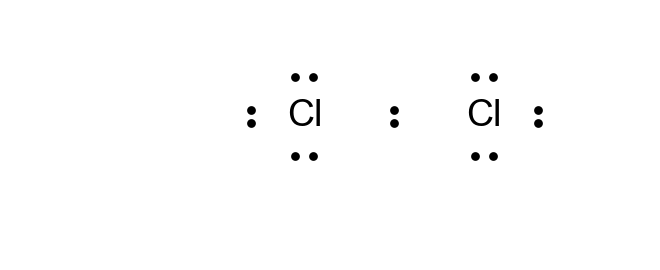
\includegraphics[width=0.86\linewidth]{rasmlar/gen/lw_231998.png}\end{center}
Molekuladagi umumiy bog`lovchi elektron juftlari \textbf{sonini aniqlang.}

\noindent A)~\textsl{2} \hfill B)~\textsl{3} \hfill C)~\textsl{1} \hfill D)~\textsl{4}\par
\vspace{4pt}
\noindent\textbf{2.} Metall oksidida kislorodning massa ulushi 28,57\%. Metallning ekvivalent \textbf{massasini (g/mol) aniqlang.}

\noindent A)~\textsl{20} \hfill B)~\textsl{40} \hfill C)~\textsl{10} \hfill D)~\textsl{30}\par
\vspace{4pt}
\noindent\textbf{3.} Jadvalda metall plastinkalarning tuz eritmalariga tushirilishidagi kuzatuvlar berilgan (``+'' -- metall ajraladi, reaksiya boradi; ``$-$'' -- reaksiya bormaydi):
\begin{center}
\renewcommand{\arraystretch}{1.15}
\begin{tabular}{|c|c|c|c|}\hline
\textbf{Metall} & \textbf{CuSO\textsubscript{4} eritmasi} & \textbf{AgNO\textsubscript{3} eritmasi} & \textbf{ZnSO\textsubscript{4} eritmasi} \\ \hline
Cu & $-$ & + & $-$ \\ \hline
Mg & + & + & + \\ \hline
Fe & + & + & $-$ \\ \hline
\end{tabular}
\end{center}
Ushbu metallardan qaysi biri eng faol?

\noindent A)~\textsl{Cu} \hfill B)~\textsl{Fe} \hfill C)~\textsl{Zn} \hfill D)~\textsl{Mg}\par
\vspace{4pt}
\noindent\textbf{4.} 12 g NaOH ni to`liq neytrallash uchun 14,7 g H\textsubscript{2}SO\textsubscript{4} sarflandi (ikkala H almashinadi). H\textsubscript{2}SO\textsubscript{4} ning ekvivalent \textbf{massasini (g/mol) aniqlang.}

\noindent A)~\textsl{98} \hfill B)~\textsl{24,5} \hfill C)~\textsl{49} \hfill D)~\textsl{14,7}\par
\vspace{4pt}
\noindent\textbf{5.} AgNO\textsubscript{3} eritmasi inert elektrodlar yordamida 5 A tok kuchi bilan 1930 s elektroliz qilindi. Katodda ajralgan Ag massasi (g) \textbf{ni toping.}

\noindent A)~\textsl{21,6} \hfill B)~\textsl{5,4} \hfill C)~\textsl{10,8} \hfill D)~\textsl{1,08}\par
\vspace{4pt}
\noindent\textbf{6.} AgNO\textsubscript{3} ning suvli eritmasi inert elektrodlar bilan elektroliz qilinganda qaysi moddalar ajraladi?

\noindent\begin{tabular}{@{}p{0.47\linewidth}@{}p{0.47\linewidth}@{}}
A)~\textsl{H\textsubscript{2}, Cl\textsubscript{2} va NaOH} & B)~\textsl{H\textsubscript{2} va O\textsubscript{2}} \\
C)~\textsl{Ag va O\textsubscript{2}} & D)~\textsl{Zn, H\textsubscript{2} va O\textsubscript{2}} \\
\end{tabular}\par
\vspace{4pt}
\noindent\textbf{7.} H\textsubscript{2}O\textsubscript{2} moddaning parchalanish reaksiyasida konsentratsiyaning vaqt bo`yicha o`zgarishi jadvalda berilgan:
\begin{center}
\renewcommand{\arraystretch}{1.15}
\begin{tabular}{|c|c|}\hline
\textbf{t, min} & \textbf{c, mol/l} \\ \hline
0 & 1,6 \\ \hline
2 & 1,28 \\ \hline
4 & 0,96 \\ \hline
6 & 0,64 \\ \hline
\end{tabular}
\end{center}
0-minutdan 4-minutgacha o`rtacha tezlikni mol/(l$\cdot$min) \textbf{hisoblang.}

\noindent A)~\textsl{0,32} \hfill B)~\textsl{0,08} \hfill C)~\textsl{0,16} \hfill D)~\textsl{0,64}\par
\vspace{4pt}
\noindent\textbf{8.} Na\textsubscript{2}CO\textsubscript{3}$\cdot$10H\textsubscript{2}O kristallogidrat namunasi (25 g) bosqichma-bosqich qizdirilganda uning massasi o`zgarishi grafikda keltirilgan.
\begin{center}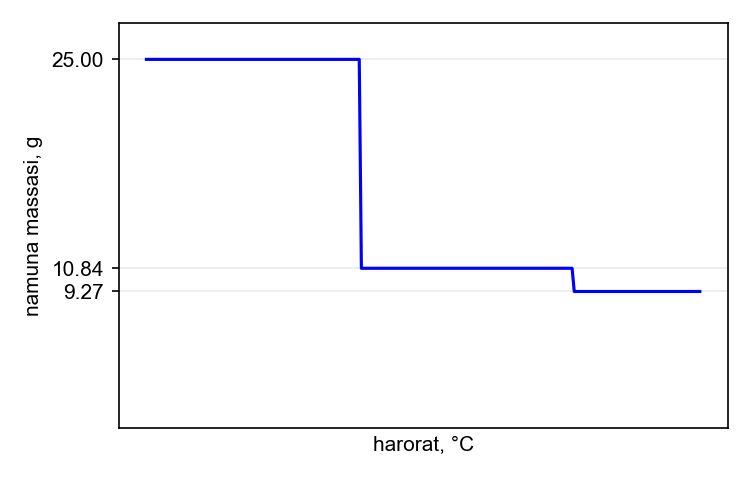
\includegraphics[width=0.86\linewidth]{rasmlar/gen/hy_v14_0.png}\end{center}
To`liq suvsizlangandan keyin qolgan Na\textsubscript{2}CO\textsubscript{3} ning \textbf{massasini (g) toping.}

\noindent A)~\textsl{9,27} \hfill B)~\textsl{15,73} \hfill C)~\textsl{10,84} \hfill D)~\textsl{18,53}\par
\vspace{4pt}
\noindent\textbf{9.} Jadvalda bog`lar hosil qiluvchi atomlarning elektrmanfiyliklari berilgan:
\begin{center}
\renewcommand{\arraystretch}{1.15}
\begin{tabular}{|c|c|c|}\hline
\textbf{Bog`} & \textbf{EM (1-atom)} & \textbf{EM (2-atom)} \\ \hline
H--F & 2,1 & 4 \\ \hline
K--Br & 0,8 & 2,8 \\ \hline
Na--Cl & 0,9 & 3 \\ \hline
H--N & 2,1 & 3 \\ \hline
\end{tabular}
\end{center}
Qaysi bog` eng qutbli (eng ko`p ionli xarakterga ega)?

\noindent A)~\textsl{H--F} \hfill B)~\textsl{Na--Cl} \hfill C)~\textsl{K--Br} \hfill D)~\textsl{H--N}\par
\vspace{4pt}
\noindent\textbf{10.} Kislorod (\textit{Z} = 8) atomining eng tashqi pog`onasidagi p-elektronlar \textbf{sonini aniqlang.}

\noindent A)~\textsl{5} \hfill B)~\textsl{4} \hfill C)~\textsl{3} \hfill D)~\textsl{6}\par
\vspace{4pt}
\noindent\textbf{11.} Gazlar aralashmasi tarkibi jadvalda berilgan (n.sh.):
\begin{center}
\renewcommand{\arraystretch}{1.15}
\begin{tabular}{|c|c|}\hline
\textbf{Gaz} & \textbf{Hajmi, l} \\ \hline
He & 3 \\ \hline
CH\textsubscript{4} & 2 \\ \hline
NH\textsubscript{3} & 3 \\ \hline
\end{tabular}
\end{center}
Aralashmaning havoga nisbatan \textbf{zichligini aniqlang} (M(havo) = 29 g/mol).

\noindent A)~\textsl{0,41} \hfill B)~\textsl{0,82} \hfill C)~\textsl{0,2} \hfill D)~\textsl{11,88}\par
\vspace{4pt}
\noindent\textbf{12.} 13,5 g Al reaksiyaga kirishdi (2Al + 6HCl $\to$ 2AlCl\textsubscript{3} + 3H\textsubscript{2}). Ajralgan H\textsubscript{2} \textbf{hajmini (l, n.sh.) hisoblang.}

\noindent A)~\textsl{33,6} \hfill B)~\textsl{8,4} \hfill C)~\textsl{11,2} \hfill D)~\textsl{16,8}\par
\vspace{4pt}
\noindent\textbf{13.} Mishyak (\textit{Z} = 33) atomining eng tashqi pog`onasidagi p-elektronlar \textbf{sonini aniqlang.}

\noindent A)~\textsl{4} \hfill B)~\textsl{3} \hfill C)~\textsl{2} \hfill D)~\textsl{5}\par
\vspace{4pt}
\noindent\textbf{14.} K va Li dan iborat 13,1 g aralashma suv bilan reaksiyaga kirishdi. Ajralgan vodorodning \textbf{hajmini (l, n.sh.) aniqlang.}

\noindent A)~\textsl{11,2} \hfill B)~\textsl{2,8} \hfill C)~\textsl{6,55} \hfill D)~\textsl{5,6}\par
\vspace{4pt}
\noindent\textbf{15.} Alyuminiy va temir dan iborat 13,7 g aralashma mo`l NaOH eritmasida eritildi. Ajralgan gazning \textbf{hajmini (l, n.sh.) aniqlang} (temir ishqor bilan reaksiyaga kirishmaydi).

\noindent A)~\textsl{10,08} \hfill B)~\textsl{20,16} \hfill C)~\textsl{5,04} \hfill D)~\textsl{11,37}\par
\vspace{4pt}
\noindent\textbf{16.} D-metallar va ularning birikmalari haqida qaysi fikrlar to`g`ri? 1) Rux eritmada Fe\textsuperscript{2+} ni siqib chiqara olmaydi; 2) Fe(OH)\textsubscript{2} havoda qo`ng`ir rangga o`tadi; 3) Cu(OH)\textsubscript{2} qizdirilganda CuO ga parchalanadi; 4) Mis nam havoda (CuOH)\textsubscript{2}CO\textsubscript{3} qoplamasi bilan qoplanadi

\noindent A)~\textsl{1, 4} \hfill B)~\textsl{1, 2, 4} \hfill C)~\textsl{2, 3} \hfill D)~\textsl{2, 3, 4}\par
\vspace{4pt}
\noindent\textbf{17.} 1 l suvda 0,02 mol Ca(HCO\textsubscript{3})\textsubscript{2}, 0,04 mol CaSO\textsubscript{4} va 0,02 mol MgCl\textsubscript{2} erigan. Suv qaynatilgandan keyin qolgan qattiqlikni yo`qotish uchun necha gramm soda (Na\textsubscript{2}CO\textsubscript{3}) kerak?

\noindent A)~\textsl{8,48} \hfill B)~\textsl{4,24} \hfill C)~\textsl{6,36} \hfill D)~\textsl{2,12}\par
\vspace{4pt}
\noindent\textbf{18.} Reaksiya tenglamasi: Al\textsubscript{2}O\textsubscript{3} + 3H\textsubscript{2}SO\textsubscript{4} $\to$ Al\textsubscript{2}(SO\textsubscript{4})\textsubscript{3} + 3H\textsubscript{2}O. Reaksiyaga 49 g H\textsubscript{2}SO\textsubscript{4} kirishdi. Al\textsubscript{2}(SO\textsubscript{4})\textsubscript{3} \textbf{massasini (g) hisoblang.}

\noindent A)~\textsl{513} \hfill B)~\textsl{57} \hfill C)~\textsl{114} \hfill D)~\textsl{28,5}\par
\vspace{4pt}
\noindent\textbf{19.} Qaysi juftliklar o`zaro reaksiyaga kirishmaydi? 1) Na\textsubscript{2}CO\textsubscript{3} va HCl; 2) ZnO va HCl; 3) Fe va HNO\textsubscript{3}(sovuq kons.); 4) Al\textsubscript{2}O\textsubscript{3} va NaOH

\noindent A)~\textsl{1, 4} \hfill B)~\textsl{2, 3} \hfill C)~\textsl{1, 2} \hfill D)~\textsl{3}\par
\vspace{4pt}
\noindent\textbf{20.} CH\textsubscript{3}--CH(NH\textsubscript{2})--CH\textsubscript{2}--CH\textsubscript{3} birikmaning sistematik nomi qaysi qatorda to`g`ri keltirilgan?

\noindent\begin{tabular}{@{}p{0.47\linewidth}@{}p{0.47\linewidth}@{}}
A)~\textsl{butan-1-amin} & B)~\textsl{butan-2-amin} \\
C)~\textsl{2-metilpropan-1-amin} & D)~\textsl{2-aminobutanol} \\
\end{tabular}\par
\vspace{4pt}
\noindent\textbf{21.} CH\textsubscript{3}--CH(CH\textsubscript{3})--CH\textsubscript{2}--OH birikmaning sistematik nomi qaysi qatorda to`g`ri keltirilgan?

\noindent\begin{tabular}{@{}p{0.47\linewidth}@{}p{0.47\linewidth}@{}}
A)~\textsl{butanol-1} & B)~\textsl{2-metilpropanol-1} \\
C)~\textsl{2-metilpropanol-2} & D)~\textsl{butanol-2} \\
\end{tabular}\par
\vspace{4pt}
\noindent\textbf{22.} C\textsubscript{6}H\textsubscript{6} + 3H\textsubscript{2} $\to$ C\textsubscript{6}H\textsubscript{12} reaksiyasida 15,6 g C\textsubscript{6}H\textsubscript{6} ishtirok etdi. C\textsubscript{6}H\textsubscript{12} \textbf{miqdorini (mol) toping.}

\noindent A)~\textsl{0,2} \hfill B)~\textsl{0,4} \hfill C)~\textsl{0,1} \hfill D)~\textsl{0,3}\par
\vspace{4pt}
\noindent\textbf{23.} C\textsubscript{2}H\textsubscript{5}OH va C\textsubscript{3}H\textsubscript{7}OH dan iborat 15,2 g aralashma natriy bilan to`liq reaksiyaga kirishganda 3,36 l (n.sh.) vodorod ajraldi. Aralashmadagi C\textsubscript{2}H\textsubscript{5}OH \textbf{massasini (g) toping.}

\noindent A)~\textsl{6} \hfill B)~\textsl{12} \hfill C)~\textsl{15,2} \hfill D)~\textsl{9,2}\par
\vspace{4pt}
\noindent\textbf{24.} Aldegid va ketonlar haqida qaysi fikrlar to`g`ri? 1) Aldegidlar "kumush ko`zgu" reaksiyasini beradi; 2) Aseton Cu(OH)\textsubscript{2} ni qaytaradi; 3) Aseton suvda erimaydi; 4) Sirka aldegid Kucherov reaksiyasi bilan olinadi

\noindent A)~\textsl{1, 4} \hfill B)~\textsl{2} \hfill C)~\textsl{4} \hfill D)~\textsl{1, 2, 4}\par
\vspace{4pt}
\noindent\textbf{25.} C\textsubscript{4}H\textsubscript{8} alkenlarning izomerlari soni (sis-trans izomerlar bilan, siklik bo`lmagan) nechta?

\noindent A)~\textsl{5} \hfill B)~\textsl{4} \hfill C)~\textsl{3} \hfill D)~\textsl{6}\par
\vspace{4pt}
\noindent\textbf{26.} CH\textsubscript{3}COOC\textsubscript{2}H\textsubscript{5} + NaOH $\to$ CH\textsubscript{3}COONa + C\textsubscript{2}H\textsubscript{5}OH reaksiyasida 8,8 g CH\textsubscript{3}COOC\textsubscript{2}H\textsubscript{5} ishtirok etdi. C\textsubscript{2}H\textsubscript{5}OH \textbf{massasini (g) toping.}

\noindent A)~\textsl{9,2} \hfill B)~\textsl{2,3} \hfill C)~\textsl{4,6} \hfill D)~\textsl{6,9}\par
\vspace{4pt}
\noindent\textbf{27.} Quyidagi birikmalardan qaysi biri amin sinfiga kiradi?

\noindent A)~\textsl{C\textsubscript{2}H\textsubscript{5}NH\textsubscript{2}} \hfill B)~\textsl{C\textsubscript{2}H\textsubscript{5}OH} \hfill C)~\textsl{C\textsubscript{6}H\textsubscript{5}OH} \hfill D)~\textsl{C\textsubscript{12}H\textsubscript{22}O\textsubscript{11}}\par
\vspace{4pt}
\noindent\textbf{28.} Aminlar, aminokislotalar va oqsillar haqida qaysi fikrlar to`g`ri? 1) Anilin bromli suv bilan oq cho`kma beradi; 2) Oqsillar biuret reaksiyasini beradi; 3) Glitsin optik faol; 4) Nitrobenzoldan anilin Zinin reaksiyasi bilan olinadi

\noindent A)~\textsl{2, 4} \hfill B)~\textsl{1, 2, 4} \hfill C)~\textsl{2, 3, 4} \hfill D)~\textsl{1, 3, 4}\par
\vspace{4pt}
\noindent\textbf{29.} Yuqori molekulyar birikmalar haqida qaysi fikrlar to`g`ri? 1) Fenolformaldegid smola polikondensatsiya mahsuloti; 2) Polietilen polimerlanish reaksiyasi bilan olinadi; 3) Teflon --- polivinilxlorid; 4) Kapron poliamid tola

\noindent A)~\textsl{1, 2, 4} \hfill B)~\textsl{1, 2} \hfill C)~\textsl{1, 3} \hfill D)~\textsl{1, 3, 4}\par
\vspace{4pt}
\noindent\textbf{30.} Eritmaga AgNO\textsubscript{3} qo`shilganda sariq cho`kma (Ag\textsubscript{3}PO\textsubscript{4}), HNO\textsubscript{3} da eriydi kuzatildi. Eritmada qaysi ion bor?

\noindent A)~\textsl{SO\textsubscript{4}\textsuperscript{2$-$}} \hfill B)~\textsl{NH\textsubscript{4}\textsuperscript{+}} \hfill C)~\textsl{Ag\textsuperscript{+}} \hfill D)~\textsl{PO\textsubscript{4}\textsuperscript{3$-$}}\par
\vspace{4pt}
\noindent\textbf{31.} Rasmdagi usul bilan qaysi moddani eritmadan ajratib olish mumkin?
\begin{center}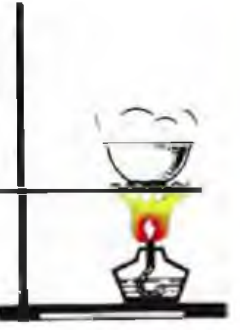
\includegraphics[width=0.86\linewidth]{rasmlar/darslik/d_bugla.png}\end{center}
\noindent A)~\textsl{kerosinni suvdan}\par
\noindent B)~\textsl{qumni suvdan}\par
\noindent C)~\textsl{osh tuzini tuz eritmasidan}\par
\noindent D)~\textsl{suvni osh tuzi eritmasidan (toza holda)}\par
\vspace{4pt}
\noindent\textbf{32.} 100 g 4\% li CuSO\textsubscript{4} eritmasini CuSO\textsubscript{4}$\cdot$5H\textsubscript{2}O dan tayyorlash uchun necha gramm kristallogidrat kerak?

\noindent\begin{tabular}{@{}p{0.47\linewidth}@{}p{0.47\linewidth}@{}}
A)~\textsl{4} & B)~\textsl{12,5} \\
C)~\textsl{3,12} & D)~\textsl{6,25   ---} \\
\end{tabular}\par
\vspace{4pt}
\end{multicols}
\medskip
\noindent\setlength{\fboxsep}{0pt}\fbox{\begin{tabular}{p{0.74\linewidth}|p{0.2\linewidth}}
\parbox[t]{0.72\linewidth}{\vspace{3pt}\textbf{Topshiriqlar (33--35) va javob variant (A--F)larini o`zaro to`g`ri moslashtiring.} Etan (C\textsubscript{2}H\textsubscript{6}) va eten (C\textsubscript{2}H\textsubscript{4}) dan iborat 8,96 l (n.sh.) aralashma bromli suvdan o`tkazilganda 16 g brom yutildi.
\vspace{3pt}} & \parbox[t]{0.19\linewidth}{\vspace{3pt}A~\textsl{1,12}\\[3pt]
B~\textsl{25}\\[3pt]
C~\textsl{144}\\[3pt]
D~\textsl{115,2}\\[3pt]
E~\textsl{2,24}\\[3pt]
F~\textsl{288}}\\ \hline
\parbox[t]{0.72\linewidth}{\vspace{2pt}\textbf{33. Aralashmadagi eten (C\textsubscript{2}H\textsubscript{4}) hajmini (l, n.sh.) aniqlang.}\vspace{2pt}} & \\ \hline
\parbox[t]{0.72\linewidth}{\vspace{2pt}\textbf{34. Aralashmadagi eten (C\textsubscript{2}H\textsubscript{4}) hajmiy ulushini (\%) aniqlang.}\vspace{2pt}} & \\ \hline
\parbox[t]{0.72\linewidth}{\vspace{2pt}\textbf{35. Aralashmani to`liq yoqish uchun zarur havo hajmini (l, n.sh.; havoda 21\% kislorod bor) aniqlang.}\vspace{2pt}} & 
\end{tabular}}
\par\bigskip
\noindent\textbf{36.} Cu + H\textsubscript{2}SO\textsubscript{4} $\to$ CuSO\textsubscript{4} + SO\textsubscript{2} + H\textsubscript{2}O reaksiya tenglamasini tenglang. Reagentlar (chap qism) koeffitsiyentlari \textbf{yig`indisini toping.}
\javob
\noindent\textbf{37.} Reaksiya 30 \textdegree{}C da 72 minutda tugaydi. $\gamma$ = 2. Harorat 30 \textdegree{}C ga oshirilib, reagentlardan birining konsentratsiyasi 2 marta oshirildi (reaksiya shu modda bo`yicha 1-tartibli). Reaksiya necha minutda tugaydi?
\javob
\noindent\textbf{38.} CaCO\textsubscript{3} va MgCO\textsubscript{3} dan iborat 36,8 g aralashma doimiy massagacha qizdirilganda qoldiq massasi 19,2 g bo`ldi. Aralashmadagi CaCO\textsubscript{3} ning \textbf{massasini (g) toping.}
\javob
\noindent\textbf{39.} 4,6 g etanol avval sirka aldegidgacha (unum 75\%), so`ng sirka kislotagacha (unum 80\%) oksidlandi; hosil bo`lgan kislota mo`l etanol bilan efirlandi (unum 100\%). Etilatsetat \textbf{massasini (g) toping.}
\javob
\noindent\textbf{40.} 61,5 g nitrobenzol anilinga qaytarildi (unum 90\%), hosil bo`lgan anilin mo`l bromli suv bilan reaksiyaga kirishdi (unum 80\%). Hosil bo`lgan 2,4,6-tribromanilin (M = 330 g/mol) \textbf{massasini (g) toping.}
\javob
\par\bigskip\begin{center}\textbf{\fontsize{13}{15}\selectfont YOZMA ISH}\end{center}
\noindent\textbf{41.} \textbf{Topshiriqni bajarish jarayonida barcha reaksiya tenglamalarini yozing. Miqdoriy va arifmetik hisoblashlarni (unga asos bo`lgan usul yoki formulani ko`rsatgan holda) uzviy ketma-ketlikda bajaring.}\par\smallskip
Quyidagi eritmalar berilgan: HCl ning 0,01 mol/l li eritmasi va NaOH ning 0,04 mol/l li eritmasi. Ularni aralashtirib, umumiy hajmi 1 l bo`lgan eritma tayyorlandi (0,6 l HCl eritmasi va 0,4 l NaOH eritmasi). Shuningdek, sirka kislotaning 0,2 mol/l li eritmasida dissotsilanish darajasi 1\%.\par
\noindent 1)Aralashtirilgandan keyingi eritmaning pH ini aniqlang.\par
\noindent 2)Dastlabki HCl eritmasining pH ini hisoblang. 1 l shu eritmadagi HCl massasini (g) ham hisoblang.\par
\noindent 3)Dastlabki NaOH eritmasining pH ini hisoblang.\par
\noindent 4)Sirka kislota eritmasidagi H\textsuperscript{+} ionlari konsentratsiyasini (mol/l) va pH ni aniqlang (lg 2 = 0,3, lg 5 = 0,7 ni ishlating). Shuningdek NaOH eritmasi 100 marta suyultirilsa pH qancha bo`ladi?\par
\noindent 5)Sirka kislotaning dissotsilanish konstantasini hisoblang (K = C$\alpha$\textsuperscript{2}/(1 $-$ $\alpha$)). Shuningdek HCl eritmasi 10 marta suyultirilsa pH necha bo`ladi?\par
\diqqat{Mazkur topshiriq kengaytirilgan javobni talab etib, uning yechilish usuli va shu usul asosidagi barcha hisoblash amallari javoblar varaqasida aks etishi lozim.}
\noindent\textbf{42.} Quyidagi o`zgarishlar zanjirida \textit{X}, \textit{Y}, \textit{Z} noma'lum organik moddalar:\par
\[\setlength{\fboxsep}{0pt}\text{CH\textsubscript{3}Cl}\xrightarrow{\text{Na}}\text{\textit{X}}\xrightarrow{\text{Cl\textsubscript{2}, yorug`lik}}\text{\textit{Y}}\xrightarrow{\text{KOH (suvli)}}\text{C\textsubscript{2}H\textsubscript{5}OH}\]
\noindent 1)CH\textsubscript{3}Cl $\to$ \textit{X} : reaksiya tenglamasini yozing; hosil bo`lgan moddani nomlang.\par
\noindent 2)\textit{X} $\to$ \textit{Y} : reaksiya tenglamasini yozing; hosil bo`lgan moddani nomlang.\par
\noindent 3)\textit{Y} $\to$ C\textsubscript{2}H\textsubscript{5}OH : reaksiya tenglamasini yozing; hosil bo`lgan moddani nomlang.\par
\diqqat{Mazkur topshiriq kengaytirilgan javobni talab etib, uning yechilish usuli va shu usul asosidagi barcha hisoblash amallari javoblar varaqasida aks etishi lozim.}
\noindent\textbf{43.} \textbf{Topshiriqni bajarish jarayonida barcha reaksiya tenglamalarini yozing. Miqdoriy va arifmetik hisoblashlarni (unga asos bo`lgan usul yoki formulani ko`rsatgan holda) uzviy ketma-ketlikda bajaring.}\par\smallskip
132,4 g Pb(NO\textsubscript{3})\textsubscript{2} qizdirilganda qisman parchalandi va qattiq qoldiq massasi 110,8 g bo`ldi. Ajralgan gazlar aralashmasi 100 g suvga to`liq yuttirildi. Qattiq qoldiqdagi PbO esa mo`l suyultirilgan H\textsubscript{2}SO\textsubscript{4} bilan reaksiyaga kiritildi.\par
\noindent 1)Parchalanish reaksiyasi tenglamasini yozing. Parchalangan Pb(NO\textsubscript{3})\textsubscript{2} ning ulushini (\%) va ajralgan gazlar umumiy hajmini (l, n.sh.) aniqlang.\par
\noindent 2)Qattiq qoldiqdagi PbO ning massa ulushini (\%) hisoblang.\par
\noindent 3)Gazlar suvga yuttirilganda hosil bo`lgan eritmadagi HNO\textsubscript{3} ning massa ulushini (\%) toping (reaksiya tenglamasini yozing).\par
\noindent 4)Qoldiqdagi PbO ni to`liq eritish uchun 20\% li H\textsubscript{2}SO\textsubscript{4} eritmasidan necha gramm kerak va hosil bo`lgan PbSO\textsubscript{4} ning massasi qancha?\par
\noindent 5)Ajralgan NO\textsubscript{2} va O\textsubscript{2} gazlari aralashmasining o`rtacha molyar massasini (g/mol) hisoblang.\par
\diqqat{Mazkur topshiriq kengaytirilgan javobni talab etib, uning yechilish usuli va shu usul asosidagi barcha hisoblash amallari javoblar varaqasida aks etishi lozim.}
\newpage
\noindent\textbf{\fontsize{13}{15}\selectfont Nazorat testi}\ \textit{$\cdot$ 14-variant}\hfill \textbf{Javoblar kaliti}\par\smallskip\hrule\smallskip
\textit{Faqat o`qituvchi uchun.}\par\medskip
\noindent\textbf{1--32-savollar}\par\smallskip
\noindent\begin{tabular}{|c|c|c|c|c|c|c|c|c|c|c|c|c|c|c|c|}\hline
\textbf{1} & \textbf{2} & \textbf{3} & \textbf{4} & \textbf{5} & \textbf{6} & \textbf{7} & \textbf{8} & \textbf{9} & \textbf{10} & \textbf{11} & \textbf{12} & \textbf{13} & \textbf{14} & \textbf{15} & \textbf{16}\\\hline
\textsl{C} & \textsl{A} & \textsl{D} & \textsl{C} & \textsl{C} & \textsl{C} & \textsl{C} & \textsl{A} & \textsl{B} & \textsl{B} & \textsl{A} & \textsl{D} & \textsl{B} & \textsl{D} & \textsl{A} & \textsl{D}\\\hline
\textbf{17} & \textbf{18} & \textbf{19} & \textbf{20} & \textbf{21} & \textbf{22} & \textbf{23} & \textbf{24} & \textbf{25} & \textbf{26} & \textbf{27} & \textbf{28} & \textbf{29} & \textbf{30} & \textbf{31} & \textbf{32}\\\hline
\textsl{C} & \textsl{B} & \textsl{D} & \textsl{B} & \textsl{B} & \textsl{A} & \textsl{D} & \textsl{A} & \textsl{B} & \textsl{C} & \textsl{A} & \textsl{B} & \textsl{A} & \textsl{D} & \textsl{C} & \textsl{D}\\\hline
\end{tabular}\par\medskip
\noindent\textbf{33--35-savollar}\par\smallskip
\noindent\begin{tabular}{|c|c|c|}\hline \textbf{No} & \textbf{Javob} & \textbf{Qiymat}\\\hline
33 & \textsl{E} & 2,24\\\hline
34 & \textsl{B} & 25\\\hline
35 & \textsl{C} & 144\\\hline
\end{tabular}\par\medskip
\noindent\textbf{36--40-savollar}\par\smallskip
\noindent\begin{tabular}{|c|c|}\hline \textbf{No} & \textbf{To`g`ri javob}\\\hline
36 & 3\\\hline
37 & 4,5\\\hline
38 & 20\\\hline
39 & 5,28\\\hline
40 & 118,8\\\hline
\end{tabular}\par\medskip
\noindent\textbf{41--43-topshiriqlar: qisqa yechim}\par\smallskip
\noindent\textbf{41-topshiriq.}\par
\noindent 1) n(H\textsuperscript{+}) = 0,006 mol; n(OH\textsuperscript{$-$}) = 0,016 mol; ortiqcha OH\textsuperscript{$-$}: 0,01 mol / 1 l = 10\textsuperscript{$-$}2 mol/l $\to$ \textbf{pH = 12}\par
\noindent 2) [H\textsuperscript{+}] = 0,01 $\to$ \textbf{pH = 2}; m = 0,01$\cdot$36,5 = \textbf{0,36 g}\par
\noindent 3) [OH\textsuperscript{$-$}] = 0,04 $\to$ pOH = 1,4 $\to$ \textbf{pH = 12,6}\par
\noindent 4) [H\textsuperscript{+}] = C$\alpha$ = 0,2$\cdot$0,01 = 0,002 mol/l $\to$ \textbf{pH = 2,7}; pH = 14 + lg(0,04/100) = \textbf{10,6}\par
\noindent 5) K = 0,2$\cdot$0,01\textsuperscript{2}/(1 $-$ 0,01) = \textbf{2,02$\cdot$10\textasciicircum{}-5}; [H\textsuperscript{+}] = 0,01/10 $\to$ \textbf{pH = 3}\par
\noindent Jami: M 15 + A 10 = 25 ball.\par
\noindent\textbf{42-topshiriq.}\par
\noindent 1) CH\textsubscript{3}Cl + Na $\to$ C\textsubscript{2}H\textsubscript{6} (etan)\par
\noindent 2) C\textsubscript{2}H\textsubscript{6} + Cl\textsubscript{2}, yorug`lik $\to$ C\textsubscript{2}H\textsubscript{5}Cl (xloretan)\par
\noindent 3) C\textsubscript{2}H\textsubscript{5}Cl + KOH (suvli) $\to$ C\textsubscript{2}H\textsubscript{5}OH (etanol)\par
\noindent Jami 25 ball.\par
\noindent\textbf{43-topshiriq.}\par
\noindent 1) 2Pb(NO\textsubscript{3})\textsubscript{2} $\to$ 2PbO + 4NO\textsubscript{2} + O\textsubscript{2}; massa kamayishi 21,6 g; parchalangan 0,2 mol, boshlang`ich 0,4 mol $\to$ \textbf{50\%}; gazlar: NO\textsubscript{2} 0,4 + O\textsubscript{2} 0,1 mol $\to$ \textbf{11,2 l}\par
\noindent 2) PbO 0,2 mol = 44,6 g; $\omega$ = 44,6/110,8 = \textbf{40,3\%}\par
\noindent 3) 4NO\textsubscript{2} + O\textsubscript{2} + 2H\textsubscript{2}O $\to$ 4HNO\textsubscript{3}: HNO\textsubscript{3} 0,4 mol = 25,2 g; eritma 100 + 18,4 + 3,2 = 121,6 g $\to$ \textbf{20,72\%}\par
\noindent 4) PbO + H\textsubscript{2}SO\textsubscript{4} $\to$ PbSO\textsubscript{4} + H\textsubscript{2}O: n(H\textsubscript{2}SO\textsubscript{4}) = 0,2 mol = 19,6 g $\to$ 20\% li eritma \textbf{98 g}; PbSO\textsubscript{4}: 0,2 mol $\cdot$ 303 = \textbf{60,6 g}\par
\noindent 5) NO\textsubscript{2} : O\textsubscript{2} = 4 : 1 $\to$ M = (4$\cdot$46 + 32)/5 = \textbf{43,2 g/mol}\par
\noindent Jami: M 15 + A 10 = 25 ball.\par
\par\bigskip\noindent\textbf{Mavzular taqsimoti}\par\smallskip
{\small\noindent\begin{longtable}{|c|p{7.2cm}|p{5.4cm}|c|}\hline \textbf{No} & \textbf{Mavzu} & \textbf{Tekshiriladigan ko`nikma} & \textbf{Ball}\\\hline
1 & 8-sinf (kovalent bog`) & Rasm bo`yicha tahlil & 1\\\hline
2 & 11-sinf (ekvivalentlar qonuni) & Hisoblash va masala yechish & 1\\\hline
3 & Tirkashev \textit{V} bob (kuchlanish qatori, jadval) & Jadval tahlili & 1\\\hline
4 & 11-sinf (ekvivalentlar qonuni) & Hisoblash va masala yechish & 1\\\hline
5 & 11-sinf 8-bob (Faradey qonunlari); Tirkashev \textit{V} bob & Hisoblash va masala yechish & 1\\\hline
6 & 11-sinf 8-bob; Tirkashev \textit{V} bob (elektroliz) & Bilim va tushunish & 1\\\hline
7 & Tirkashev VI bob (tezlik, jadval) & Jadval tahlili & 1\\\hline
8 & 7-sinf (kristallogidratlar) & Grafik tahlili & 1\\\hline
9 & 8-sinf (kimyoviy bog`lanish turlari, jadval) & Jadval tahlili & 1\\\hline
10 & Tirkashev I bob (kvant sonlari) & Bilim va tushunish & 1\\\hline
11 & 11-sinf (gaz aralashmalar, jadval) & Jadval tahlili & 1\\\hline
12 & 8-sinf; 9-sinf (stexiometriya) & Hisoblash va masala yechish & 1\\\hline
13 & Tirkashev I bob (kvant sonlari) & Bilim va tushunish & 1\\\hline
14 & 9-sinf (ishqoriy metallar) & Hisoblash va masala yechish & 1\\\hline
15 & 9-sinf (alyuminiy) & Hisoblash va masala yechish & 1\\\hline
16 & 9-sinf; Tashev (Fe, Cu, Zn, Cr) & Bilim va tushunish & 1\\\hline
17 & 9-sinf \S{}24 (doimiy qattiqlik, soda) & Hisoblash va masala yechish & 1\\\hline
18 & 9-sinf; Tirkashev (oksid/asos/kislota/tuz, hisob) & Hisoblash va masala yechish & 1\\\hline
19 & 9-sinf; Tashev (anorganik birikmalar xossalari) & Bilim va tushunish & 1\\\hline
20 & 10-sinf (nomenklatura \S{}6, \S{}11, \S{}20, \S{}24--26) & Bilim va tushunish & 1\\\hline
21 & 10-sinf (nomenklatura \S{}6, \S{}11, \S{}20, \S{}24--26) & Bilim va tushunish & 1\\\hline
22 & 10-sinf (aren, hisob) & Hisoblash va masala yechish & 1\\\hline
23 & 10-sinf \S{}21 & Hisoblash va masala yechish & 1\\\hline
24 & 10-sinf (mavzuga oid paragraflar); Abdusamatov & Bilim va tushunish & 1\\\hline
25 & 10-sinf \S{}6, \S{}12, \S{}20, \S{}28 (izomeriya) & Bilim va tushunish & 1\\\hline
26 & 10-sinf (efir, hisob) & Hisoblash va masala yechish & 1\\\hline
27 & 10-sinf (organik birikmalar sinflari) & Bilim va tushunish & 1\\\hline
28 & 10-sinf (mavzuga oid paragraflar); Abdusamatov & Bilim va tushunish & 1\\\hline
29 & 10-sinf (mavzuga oid paragraflar); Abdusamatov & Bilim va tushunish & 1\\\hline
30 & 9-sinf (sifat reaksiyalar) & Bilim va tushunish & 1\\\hline
31 & 7-sinf (12-rasm) & Rasm bo`yicha tahlil & 1\\\hline
32 & Tirkashev III bob; 7-sinf (eritma tayyorlash) & Hisoblash va masala yechish & 1\\\hline
33--35 & Aralash masala (moslashtirish) & Ko`p bosqichli hisob & 3\\\hline
36--40 & Qisqa javobli masalalar & Hisoblash & 5\\\hline
41--43 & Yozma ish & Usul va hisob (M, A) & 75\\\hline
\end{longtable}}
\end{document}
